\documentclass[a4paper,twoside,openleft]{book}
\usepackage[a4paper]{geometry}
\usepackage[utf8]{vietnam}
\usepackage{tikz}
\usetikzlibrary{calc}
\usepackage[shortlabels]{enumitem}
\usepackage{oplotsymbl,fontawesome}
\usepackage{tikz-3dplot}
\usetikzlibrary{calc,angles,fadings,decorations.text,intersections,backgrounds}
\usepackage{marvosym}
\usepackage{qrcode}
\usepackage{miama}
\tikzfading[name=fade top,
  top color=transparent!75,bottom color=transparent!0,middle color=transparent!30]
  \tikzfading[name=fade bot,
   top color=transparent!0,bottom color=transparent!95,middle color=transparent!40]
%\definecolor{xanh}{HTML}{00CC99}
\definecolor{xanh}{HTML}{24A0C2}
\definecolor{nhat}{HTML}{24C295}
\definecolor{do}{HTML}{C24624}
\definecolor{tim}{HTML}{C224A0}
\usepackage[linkcolor=xanh,colorlinks]{hyperref}
\begin{document}
\thispagestyle{empty}
\begin{tikzpicture}[overlay,remember picture,transform shape,declare function={a=20; b=9;}]
\clip (current page.north west) coordinate (A) 
		rectangle (current page.south east) coordinate (C);
\path (current page.north east) coordinate (D) 
		(current page.south west) coordinate (B) 
		($ (A)!0.5!(D) $) coordinate (AD)
		($ (A)!0.5!(B) $) coordinate (AB)
		($ (C)!0.5!(B) $) coordinate (CB)
		($ (C)!0.5!(D) $) coordinate (CD)
		($ (A)!0.5!(C) $) coordinate (AC)
		;

%%Gốc trên bên phải, dày vòng tròn
\path[fill=xanh!65] (A)--++(0,-a)--+(a,a)--cycle;
\path[fill=xanh,path fading=fade top,fading angle=45] (A)--++(0,-a)--+(a,a)--cycle;
\begin{scope}[shift={($(A)+({0.5*a},{-0.5*a}) $)}]
	\fill[white] (0,0) circle (7.2);
	\fill[gray!15] (45:7.2) arc (45:-135:7.2)--cycle;
	\fill[gray!10] (0,0) circle (5.2);
	\fill[xanh,even odd rule]  
		(0,0) circle (6.25)  (0,0) circle (6.1)
		(0,0) circle (5.2)  (0,0) circle (4.7)
		(0,0) circle (4.5)  (0,0) circle (3.5);
	\fill[xanh] (45:6.4) arc (45:-135:6.4)--(-135:5.9)
		 arc (-135:45:5.9)--cycle;
\end{scope}

%%Gốc dưới bên phải, dãy vòng tròn
\fill[xanh,even odd rule,shift={($(C)+({-0.5*b},{0.5*b}) $)}]  (0,0) circle (2.9)  (0,0) circle (3.025);===
\path[fill=xanh!65] (C)--++(0,b)--+(-b,-b)--cycle;
\path[fill=xanh,path fading=fade bot,fading angle=45] (C)--++(0,b)--+(-b,-b)--cycle;
\begin{scope}[shift={($(C)+({-0.5*b},{0.5*b}) $)}]
	\fill[white] (0,0) circle (2.8);
	\fill[gray!15] (45:2.6) arc(45:225:2.6)--cycle;
	\fill[xanh,even odd rule](0,0) circle (2.4)  (0,0) circle (2.2);
	\fill[xanh] (0,0) circle (1.8);
\end{scope}

%%Thay thế logo ở đây. Nếu logo bằng ảng thì dùng lệnh \includegraphics[width=2.5cm]{Tên file}
\path ($ (A)+(2.5,-1.5) $) node[scale=0.35] (NL) {
\begin{tikzpicture}[declare function={r =5;rl=r*sqrt(3);
        rn=rl-r;ts=rn/r;},line join=miter,line cap=butt,color=xanh!85!black,x=0.5cm,y =0.5cm]
  \def\duong{(90:r) arc (150:270:r)
    arc(30:150:r)
    arc(270:390:r)--cycle;}
  \foreach \tl/\mau/\net in {0.385/1/3,0.625/0.8/4.5,1/0.65/5.5}{
      \begin{scope}[scale=\tl,opacity=\mau,blend mode=darken]
        \path[draw,line width=\net pt]
        \duong;
        \path[rotate=60,scale=ts,draw,line width=\net pt]
        \duong;
      \end{scope}
    } 
\end{tikzpicture}
};

%%Dòng thông tin Cơ sở ở trên
\path ($ (NL) + (1,0)$) node[anchor=west,font=\bfseries\sffamily\LARGE\color{white}]{THEME LATEX AND RELATED TOPICS};

%%Thông tin tài liệu
\path ($ (A) - (-2,18.5)$) node[anchor=west,font=\bfseries\sffamily\fmmfamily \Huge\color{tim}] (NCD){Chuyên đề};
\path ($ (NCD.south west) +(0,-0.5)$) node[anchor=west,font=\fontsize{29pt}{0pt}\fontfamily{ugq}\bfseries\selectfont]{ĐỊNH LÝ VI-ET VÀ ỨNG DỤNG};

\path ($ (B)+(3,9)$) node[anchor=north west,font=\bfseries\sffamily\Large]{
\begin{minipage}{0.75\linewidth}
	\begin{itemize}[label=\protect{\color{xanh}\rhombusdot}]
		\item Trích xuất từ các đề thi tuyển 10
		\item Đáp ứng nhiều mức độ
		\item Phân dạng chi tiết
	\end{itemize}
\end{minipage}
};

%%Năm xuất bản
\path ($ (CB) +(-3,1.75)$) node[font=\bfseries\sffamily\Large\color{xanh!80!black}]{ĐỒNG THÁP \textendash\ 4/2023};

%%Mã QR trong gốc dưới
\hypersetup{urlcolor=xanh}
\path ($ (C) + ({-0.5*b},{0.5*b})$) node[fill=white,rounded corners=1pt,outer sep=0.2pt,inner sep=2pt]{\qrcode[height=2cm]{https://forms.gle/DVpNXZAztZV8e5k4A}}; 


%%Minh họa parabol, có thể thay đổi
\path ($ (A)+(10,-10) $) node{
		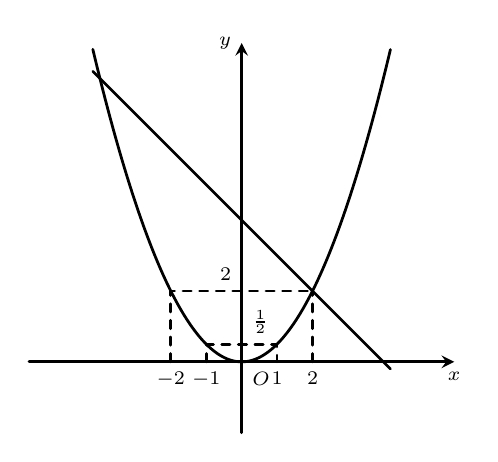
\begin{tikzpicture}[>=stealth,x=0.45cm,y=0.45cm,font=\scriptsize,line width=1pt,line cap=round]
		\draw[->] (-6,0) -- (6,0) node[below] {$x$};
		\draw[->] (0,-2) -- (0,9) node[left] {$y$};
		\draw (0,0)node[below right]{$O$};
		\draw[samples=150,smooth,domain=-4.2:4.2] plot(\x,{0.5*(\x)^2}) ;
		\draw[samples=150,smooth,domain=-4.2:4.2] plot(\x,{-(\x)+4}) ;
		\draw[dashed]
		(-2,0) node[below]{$-2$}--(-2,2)--(0,2) node[above left]{$2$}--(2,2)
		(2,0) node[below]{$2$}--(2,2)
		(-1,0) node[below]{$-1$}--(-1,0.5)--(0,0.5) node[above right]{$\frac{1}{2}$}--(1,0.5)--(1,0) node[below]{$1$};
	\end{tikzpicture}
};
\end{tikzpicture}
\end{document}